\documentclass[a4paper,11pt,listof=numbered,glossary=totoc,parskip=half,toc=bib]{scrreprt}
\usepackage[a4paper,left=2cm,right=2cm,top=2cm,bottom=2cm]{geometry}
\usepackage[onehalfspacing]{setspace}


\usepackage[colorlinks,
pdfpagelabels,
pdfstartview = FitH,
bookmarksopen = true,
bookmarksnumbered = true,
linkcolor = black,
plainpages = false,
hypertexnames = false,
citecolor = black]{hyperref}

\usepackage[utf8]{inputenc}
\usepackage[T1]{fontenc}
\usepackage[ngerman]{babel}
\usepackage{graphicx}
\usepackage{caption}
\usepackage[automake,toc,section=section,numberedsection]{glossaries}
\usepackage{uarial}
\usepackage{tabularx}
\usepackage{booktabs}
\usepackage{multirow}
\usepackage[cache=false]{minted}
\renewcommand{\listoflistingscaption}{Verzeichnis der Code-Listings}
\usepackage[table]{xcolor} % Zum Ändern der Farben in Tabellen

\usepackage{csquotes}
\usepackage[backend=biber, style=apa]{biblatex}
\addbibresource{quellen.bib}

\renewcommand{\familydefault}{\sfdefault}

\RedeclareSectionCommand[
beforeskip = 3pt,
afterskip = 3pt]{subsection} %vor subsection 6pt und nach subsection 6pt Abstand
\RedeclareSectionCommand[
beforeskip = 1pt,
afterskip = 1pt]{subsubsection} %vor subsection 6pt und nach subsection 6pt Abstand


% Glossar
\newacronym{saas}{SaaS}{Software-as-a-Service}
\newacronym{re}{RE}{Requirements Engineering}
\newacronym{qs}{QS}{Qualitätssicherung}
\newacronym{gui}{GUI}{Graphical User Interface}
\newacronym{ota}{OTA}{Over-The-Air}
\newacronym{http}{HTTP}{Hypertext Transfer Protocol}
\newacronym{jsx}{JSX}{JavaScript XML}
\newacronym{json}{JSON}{JavaScript Object Notation}
\newacronym{api}{API}{Application Programming Interface}
\newacronym{html}{HTML}{Hypertext Markup Language}
\newacronym{ux}{UX}{User Experience}
\newacronym{ui}{UI}{User Interface}
\newacronym{xml}{XML}{Extensible Markup Language}
\newacronym{css}{CSS}{Cascading Style Sheets}
\newacronym{js}{JS}{JavaScript}
\newacronym{jit}{JIT}{Just-In-Time}
\newacronym{aot}{AOT}{Ahead-Of-Time}
\newacronym{cpu}{CPU}{Central Processing Unit}
\newacronym{io}{IO}{Input / Output}
\newacronym{gpu}{GPU}{Graphics Processing Unit}
\newacronym{vm}{VM}{Virtual Machine}
\newacronym{ide}{IDE}{Integrated Development Environment}	
\newacronym{adb}{ADB}{Android Debug Bridge}
\newacronym{etl}{ETL}{Extract, Trans	form, Load}
\newacronym{dwh}{DWH}{Data Warehouse}
\newacronym{hdfs}{HDFS}{Hadoop File System}
\newacronym{crm}{CRM}{Customer Relationship Management}
\newacronym{erp}{ERP}{Enterprise Resource Planning}
\newacronym{mvp}{MVP}{Minimum Viable Product}
\newacronym{ig}{i.G.}{in Gründung}
\newacronym{ci}{CI}{Continuous Integration}
\newacronym{ssh}{SSH}{Secure Shell}
\newacronym{cd}{CD}{Continuous Delivery}
\newacronym{rest}{REST}{Representational State Transfer}
\newacronym{orm}{ORM}{Object-Relational Mapper}
\newacronym{dom}{DOM}{Document Object Model}
\newacronym{url}{URL}{Uniform Resource Locator}
\glsaddall

\makeglossaries

\subject{Meilensteinbericht}
\title{Meilenstein 1}
\subtitle{Projektkonfiguration abgeschlossen und bereitgestellt}

\begin{document}
	\pagenumbering{Roman}
	\begin{titlepage}
		
		\centering
		\vspace*{2.5cm}
		{\large\bfseries Meilensteinbericht\par}	
		{\Huge\bfseries Meilenstein 1\par}
		{\Large\bfseries Projektkonfiguration abgeschlossen und bereitgestellt\par}

		{\Large Projektteam \frqq{}Q-Teams\flqq{}\par}
		{\large\today\par}
		\vspace{0.5cm}

			
		
		
\includegraphics[scale=0.5]{iubh_logo}
		
		IUBH Fernstudium
		\vspace{0.5cm}
		
		\begin{tabular}{lllrl}
			\toprule
			\textbf{Gruppe} & \textbf{Nachname} & \textbf{Vorname} & \textbf{Matrikelnr.} & \textbf{Studiengang} \\
			\midrule
			Projektleiter & Sawatzki & Jörg & 9186524 & BSc. Informatik \\
			Mitglied 2 & Hahn & Maximilian & 91710055 & BSc. Wirtschaftsinformatik \\
			Mitglied 3 & Lapenat & Holger & 3191237 & BSc. Wirtschaftsinformatik \\
			Mitglied 4 & Moch & Daniel & 91710824 & BSc. Wirtschaftsinformatik \\
			\bottomrule
		\end{tabular}	
	\end{titlepage}
	
	
	\newpage
	\setcounter{tocdepth}{1}
	\tableofcontents
	\newpage

	\pagenumbering{arabic}	

	\chapter{Projektvision}
	
	Ein Fernstudium bedeutet meist, viele Stunden alleine lernen zu müssen. Doch dabei ist der Mensch ein ausgeprägt soziales Wesen und Kooperation sowie soziale Eingebundenheit sind wesentliche Gelingensfaktoren für einen nachhaltigen Lernprozess. Durch Kommunikation beim Lernen kann neues Wissen gesichert und vertieft werden. Inzwischen stellt dank der fortschreitenden technischen Vernetzung auch die audiovisuelle Kommunikation zwischen weltweit verteilten Menschen kein Problem mehr dar. Dennoch werden diese Potenziale derzeit nur unzureichend von Bildungseinrichtungen ausgeschöpft.
Des Weiteren verhelfen harte Fakten und Qualifikation alleine schon lange nicht mehr zu beruflichem Erfolg. Gefragt sind \textit{Soft Skills}, die aktiv zu entwickeln sind. Es gilt also: Gemeinsam lernt man am besten!

Inspiriert durch das Konzept des \frqq{}Haus des Fragens\flqq{} \autocite{HausDesFragens} machen wir mit unserem Quiz-Projekt kooperative Lernmethoden aus dem Unterrichtsraum mit Hilfe einer Webanwendung im Fernstudium nutzbar. Dabei werden in Kleingruppen kollaborativ Fragen gestaltet und kooperativ Lösungen erarbeitet. Die Fragen und Antworten werden in einem für alle Studenten zugänglichen Katalog aufgenommen, somit können Lerner jederzeit auf das gemeinsam Erarbeitete zurückgreifen und davon profitieren. Spielerische Elemente (engl. \textit{Gamification}) fördern den Spaß und die Motivation beim Lernen. Beispielsweise spornen fakultative kompetitive Elemente die Spieler zu Höchstleistungen an. Unsere Anwendung bildet den Nukleus für eine weitreichende Implementation kooperativer Lernmethoden im Fernstudium.

Das Projekt wird durch ein verteilt arbeitendes Team von vier Studenten ohne Finanzierung durchgeführt. Das Ergebnis ist die prototypische Darstellung der angeführten Funktionalitäten, eine Einbindung in das Produktivsystem der IUBH wird allerdings nicht vollzogen.
\newpage
	\chapter{Vorstellung des Teams}
	Das Projekt wird von einem vierköpfigen Team aus Studenten der Studiengänge Informatik und Wirtschaftsinformatik durchgeführt (Abbildung \ref{fig:team}). Alle Mitglieder haben beruflich bedingt unterschiedliche Vorerfahrungen und Schwerpunkte im Bereich des Software-Engineerings.

	\begin{figure}
		\centering
		
\includegraphics[width=0.2\linewidth]{Bild-Max.jpg}
		
\includegraphics[width=0.2\linewidth]{Bild-Holger-square.jpg}
		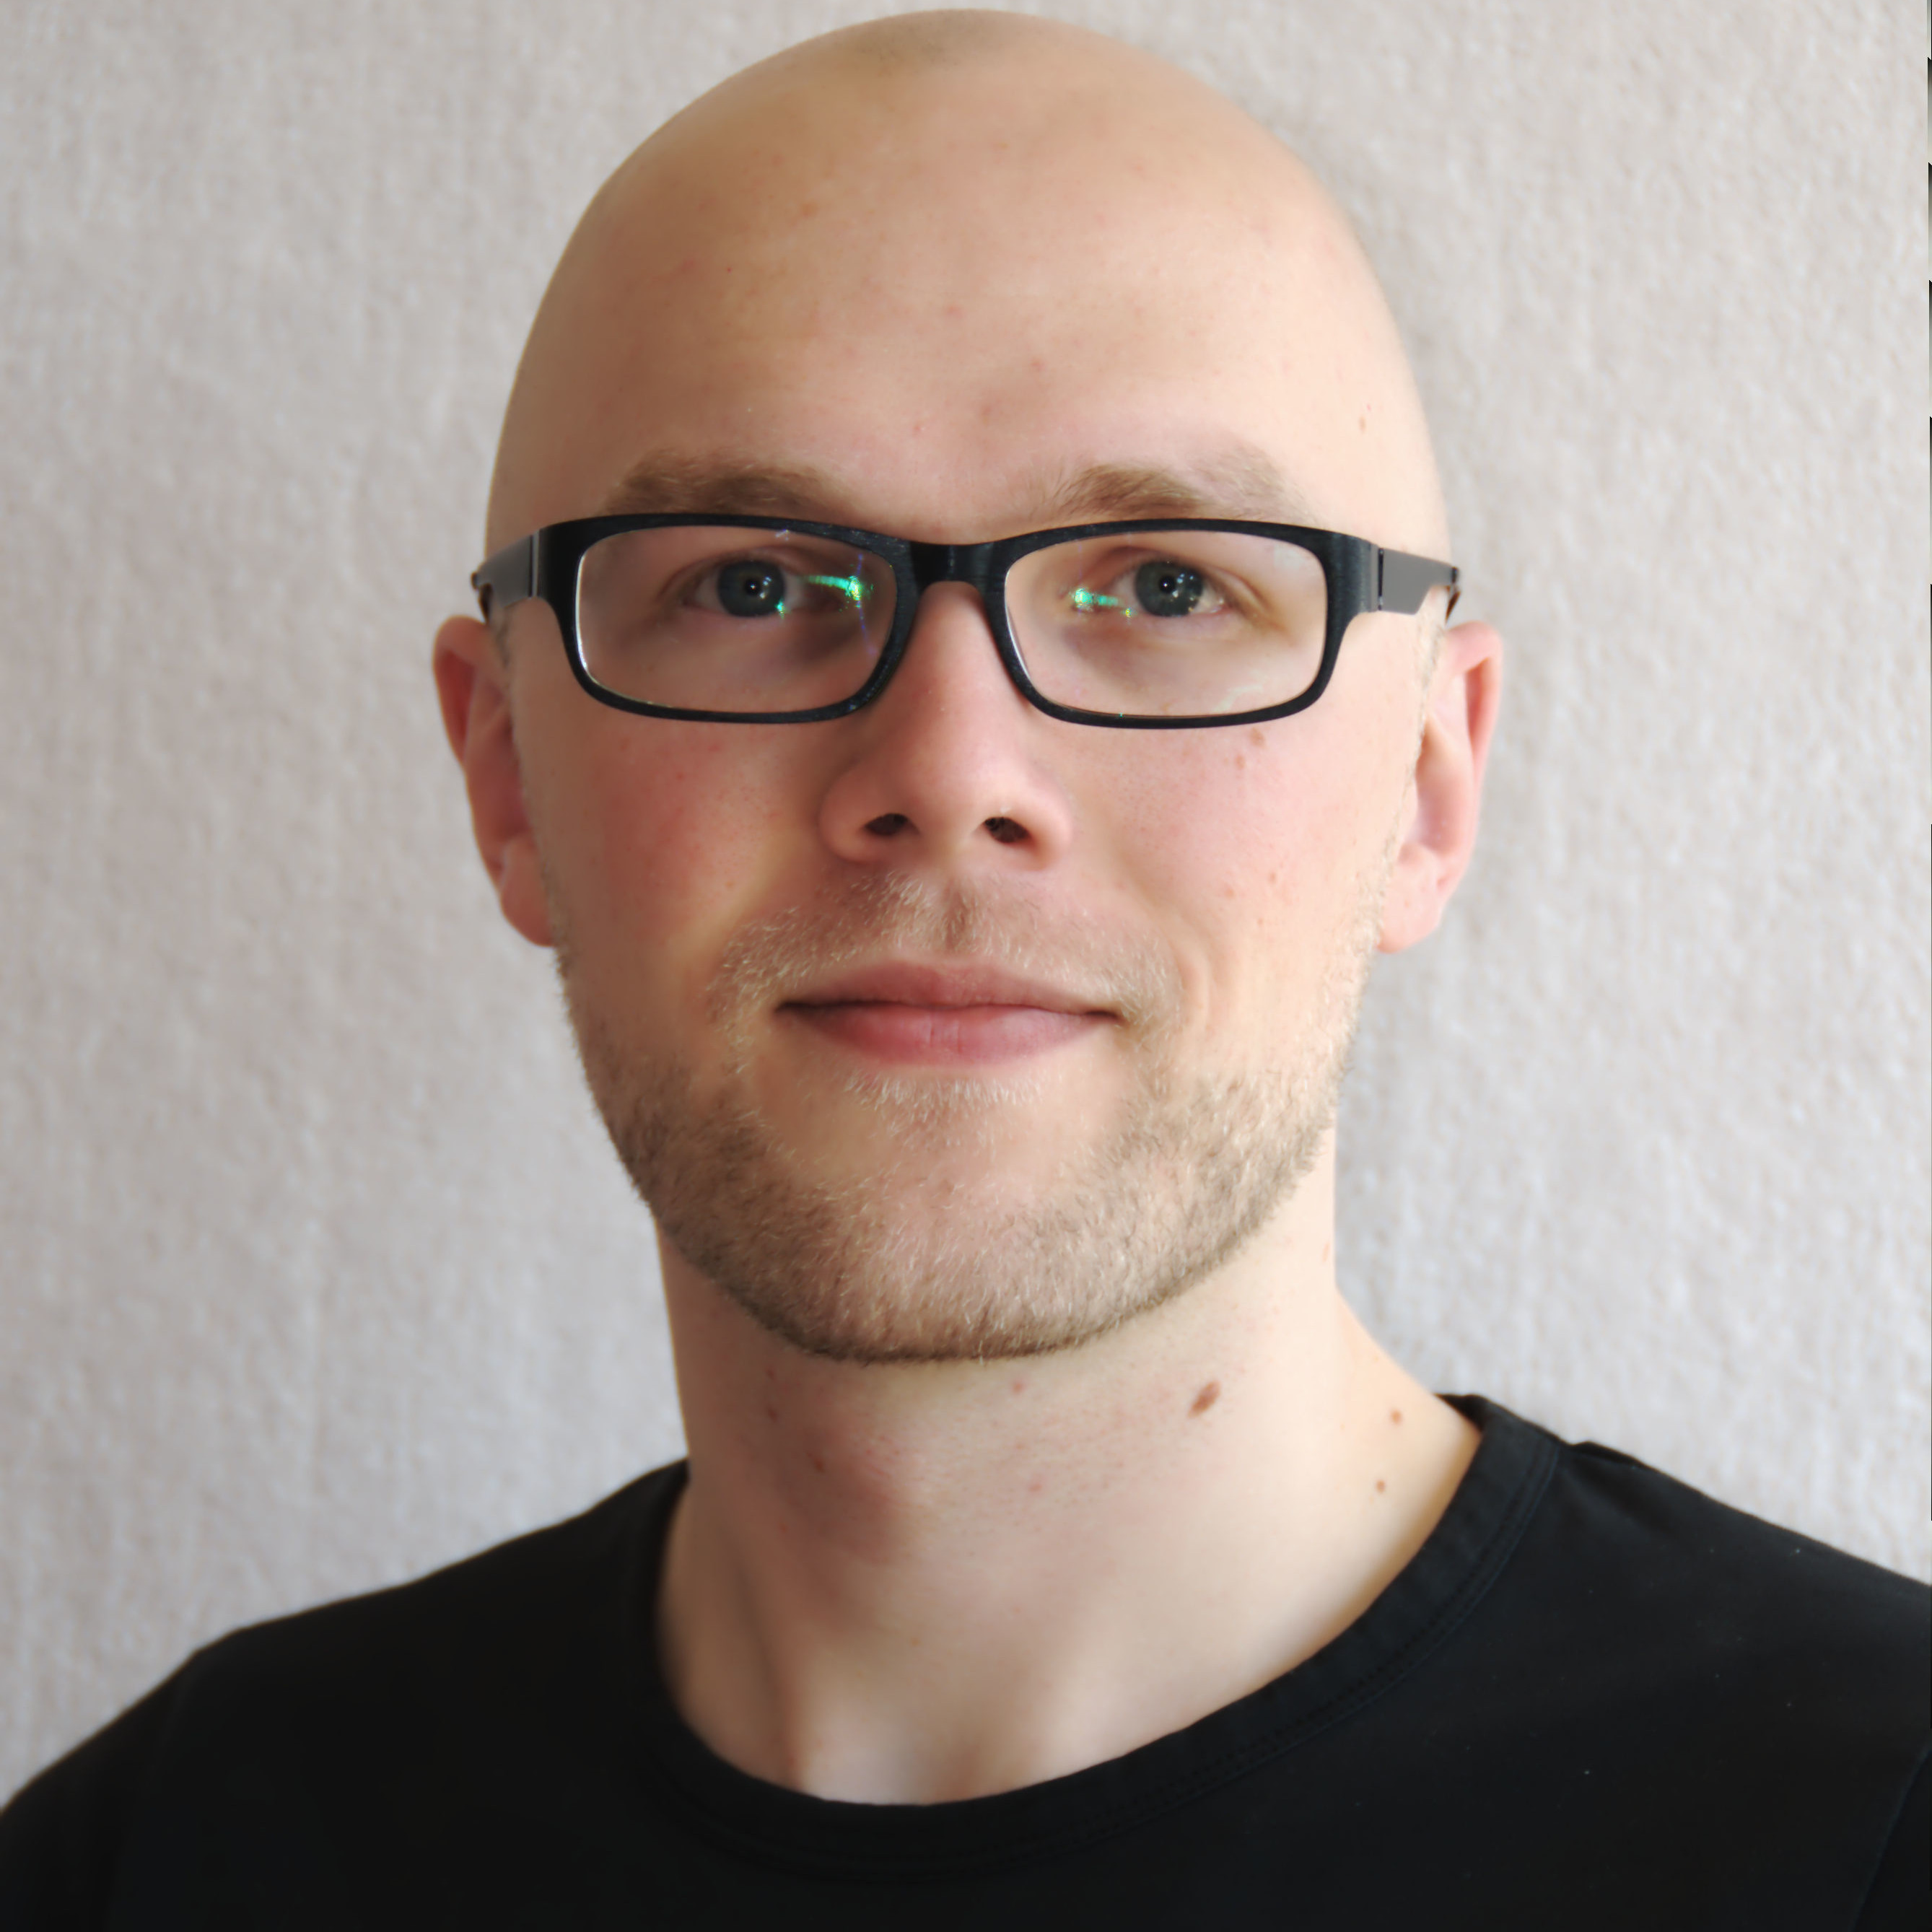
\includegraphics[width=0.2\linewidth]{Bild-Daniel-square.jpg}
		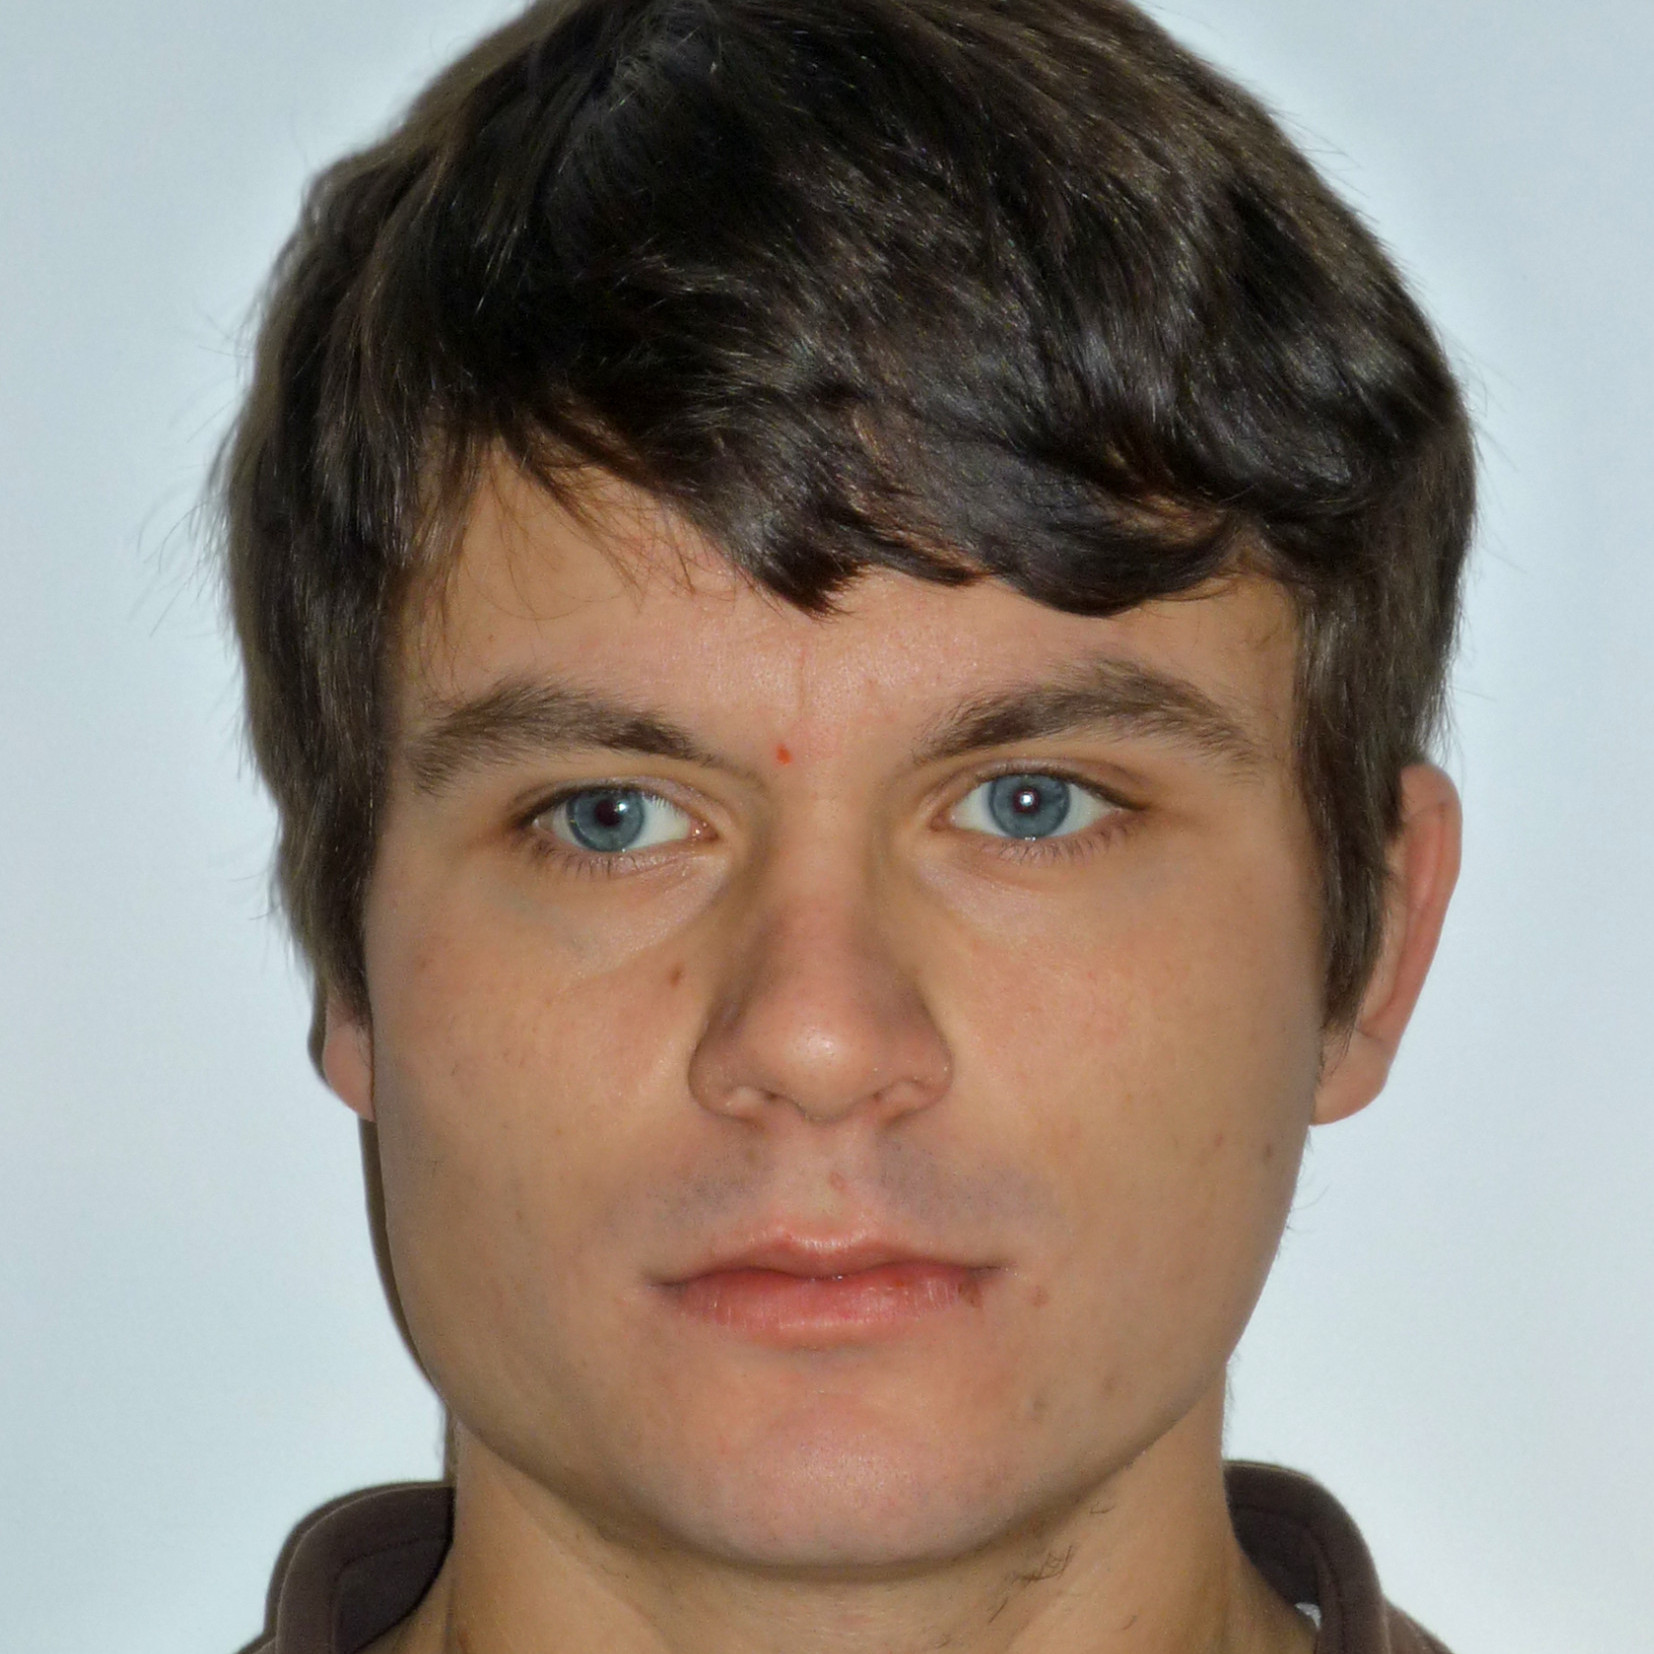
\includegraphics[width=0.2\linewidth]{Bild-Joerg-square.jpg}
		\caption{Projektteam (v.l.n.r. Maximilian Hahn, Holger Lapenat, Daniel Moch, Jörg Sawatzki)}
		\label{fig:team}
	\end{figure}


\section{Maximilian Hahn}

\begin{tabularx}{\linewidth}{lX}
\toprule
\textit{Studiengang}: & BSc. Wirtschaftsinformatik\\
\textit{Profil}: & Abgeschlossene Berufsausbildung als Zollbeamter im mittleren Dienst, Abitur nachgeholt und jetzt in der Schweiz arbeitend mit parallelem Wirtschaftsinformatik Vollzeitstudium. Arbeitet gerne im Team und lernt neue Sachen. Sportbegeistert. \\
\textit{Skills}: & Kleinere private Python Programmierungsprojekte durchgeführt; WI-Studium bis Semester 4 abgeschlossen \\
\bottomrule
\end{tabularx}

\section{Holger Lapenat}

\begin{tabularx}{\linewidth}{lX}
\toprule
\textit{Studiengang}: & BSc. Wirtschaftsinformatik\\
\textit{Profil}: & Mittlerweile über 10 Jahre Berufserfahrung in der IT. Ausbildung als Fachinformatiker Systemintegration. Privat am Wochenende sehr oft in Süddeutschland wegen Freunden und Familie unterwegs.
 \\
\textit{Skills}: & ITIL; diverse Microsoft-Zertifizierungen \\
\bottomrule
\end{tabularx}

\section{Daniel Moch}

\begin{tabularx}{\linewidth}{lX}
\toprule
\textit{Studiengang}: & BSc. Wirtschaftsinformatik\\
\textit{Profil}: & Technischer Offizier in einem binationalen Fernmeldeverband der Bundeswehr. M.Sc. Fahrzeugtechnik in 2013 abgeschlossen, 2017 Fortbildung zum Sicherheitsingenieur. Privat als Bassist in einer Band.
 \\
\textit{Skills}: & PRINCE2-Practitioner; SCRUM-Master \\
\bottomrule
\end{tabularx}

\section{Jörg Sawatzki}

\begin{tabularx}{\linewidth}{lX}
\toprule
\textit{Studiengang}: & BSc. Informatik\\
\textit{Profil}: & Selbstständiger Software-Entwickler aus Leidenschaft mit Fokus auf Projekte kleiner Startup-Unternehmen.  Privat ambitionierter Einrad- und Zweiradfahrer, Läufer, Polyglot und Globetrotter. 
 \\
\textit{Skills}: & Agiles Projektmanagement; Full-Stack-Web-Entwicklung \\
\bottomrule
\end{tabularx}
\newpage


	\chapter{Projektauftrag}

	\section{Anforderungen}

Der Software-Engineering-Prozess ist dadurch gekennzeichnet, dass er ein iterativer, kooperativer und inkrementeller Prozess ist.

Dies gilt somit auch für den Teilprozess der Anforderungsermittlung (Requirements Engineering).
Das bedeutet, dass auch das Ermitteln, Dokumentieren und Prüfen/Abstimmen der Anforderungen in mehreren Zyklen durchgeführt wird. Somit sind zu keinem Zeitpunkt im Projekt alle Anforderungen vollständig bekannt und detailliert.

Im Projektverlauf werden, bedingt durch die erkenntnisgetriebene Natur des Entwicklungsprozesses, laufend neue Anforderungen hinzu kommen und bekannte Anforderungen detailliert, verworfen oder repriorisiert werden müssen. 

Dementsprechend stellt dieser Abschnitt lediglich eine Momentaufnahme der in der Anfangsphase des Projektes ermittelten wesentlichen Anforderungen dar. Der Detailgrad der dokumentierten Anforderungen ist dementsprechend relativ niedrig gewählt, aber ausreichend, um dem Team und dem Auftraggeber einen soliden Gesamtüberblick zu vermitteln.

Das Team hat sich für die Dokumentationsform der User Stories als wichtigstes Werkzeug bei der Anforderungsermittlung entschieden. Diese wurden nach der MoSCoW-Methode bereits grob priorisiert.

\subsection{Systemkontext}

Das geplante System wird lediglich prototypisch umgesetzt, daher wird die Einbindung in die Anwendungslandschaft der IUBH zunächst nicht berücksichtigt.
Dementsprechend liegen zum aktuellen Zeitpunkt keine Schnittstellen zu Umsystemen vor.
Auch Dokumente wie z.B. rechtliche Vorschriften zum Datenschutz, liegen aktuell außerhalb des Systemkontexts.
Wichtigste Quelle von Anforderungen sind daher im wesentlichen die im folgenden Abschnitt beschriebenen Anspruchsgruppen.

\subsection{Stakeholder}

Bevor mit der Ermittlung der Anforderungen begonnen werden kann, müssen die Anspruchsgruppen (Stakeholder) ermittelt werden.

\subsubsection{Auftraggeber (Tutor)}

Der Auftraggeber ist Quelle wichtiger und verbindlicher Anforderungen, die er durch den Projektleitfaden und die themenbezogene Aufgabenstellung dem Team mitteilt.
Er ist bei wichtigen Entscheidungen einzubeziehen und muss regelmäßig über den Projektstatus informiert werden.

\subsubsection{Projektteam}

Das Team übernimmt die Verantwortung für die erfolgreiche und termingerechte Durchführung des Projektes gegenüber dem Auftraggeber.
Die Teammitglieder nehmen verschiedene Rollen an, darunter z.B. die des Entwicklers, Testers, Qualitätsmanagers oder Projektleiters. 
An jede Rolle sind verschiedene Interessen und Verantwortungen geknüpft, so dass jede Rolle eine wichtige Anforderungsquelle darstellt.

\subsubsection{Anwender}

Als Anwender sollen hier diejenigen bezeichnet werden, die das Quizsystem aktiv z.B. in der Rolle der Spieler benutzen. In der Regel handelt es sich dabei um Studierende der IUBH, die mithilfe des Quiz Lerninhalte spielerisch erarbeiten. 
Sie sind Hauptzielgruppe der Anwendung und damit eine der wichtigsten Quellen für Anforderungen, denn an ihre Akzeptanz des Produktes ist der Erfolg des Projektes eng gekoppelt. 

\subsubsection{Administrative Nutzer}

Unter diesem Begriff sind Nutzer zu verstehen, die das Quiz-System nicht aktiv nutzen, sondern lediglich administrative Aufgaben übernehmen.
Bzgl. dieser Nutzergruppe sind zum einen keine Vorgaben vom Auftraggeber gemacht worden und zum anderen ist der Lösungsansatz des Projektteams so konzipiert, dass das System kollaborativ von den Nutzern verwaltet wird. 
Somit fallen sehr wenige administrative Aufgaben an und diese Anspruchsgruppe wird nur am Rande berücksichtigt.

\subsubsection{Betreiber}

Unter den Begriff des Betreibers werden diejenigen Personen gefasst, die mit der Installation, dem Betrieb und der Wartung der Infrastruktur konfrontiert sind.
Sie müssen einen reibungslosen Betriebsablauf garantieren können und solten dementsprechend als Anforderungsquelle einbezogen werden.

\subsection{Ermittelte Anforderungen }

Dieser Abschnitt soll sich auf die vom Auftraggeber bereitgestellten Anforderungen beschränken. Das Projektteam pflegt eine umfangreiche Liste mit User Stories, die die vorgegebenen Anforderungen verfeinern und ergänzen. Sie ist in Form einer Google-Tabelle hinterlegt und wird laufend aktualisiert\footnote{https://docs.google.com/spreadsheets/d/1\_{}oWCU0Z0ybt4eHaNSfDKxIm69L42qAAZPqFLbNwvmyo/edit\# gid=0}.

\subsection{Funktionale Anforderungen}

Abbildung \ref{fig:ucd} zeigt die beiden wesentlichen fachlichen Anwendungsfälle des Systems.

\begin{figure}
	\centering
	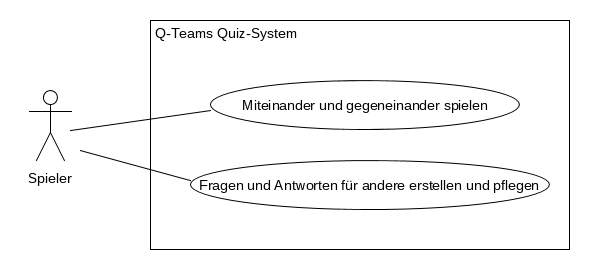
\includegraphics[width=0.8\linewidth]{ucd.png}
	\caption{Anwendungsfalldiagramm (engl. \textit{use case diagram}) des Systems}
	\label{fig:ucd}
\end{figure}

Als Spieler möchte ich mit dem Quizsystem gezielt fachliche Inhalte wiederholen, um mich auf Prüfungen vorzubereiten.

Als Spieler möchte ich gegen einen anderen Spieler antreten können, um mich mit ihm zu messen / vergleichen.

Als Spieler möchte ich mit einem anderen Spieler gemeinsam spielen, um mich im Team über Lerninhalte austauschen zu können.

Als Spieler möchte ich Fragen und Antworten für andere Spieler hinzufügen und pflegen, um mein Wissen weiterzugeben und zu festigen.

Als Spieler möchte ich Feedback zu meiner Lösung bekommen, um aus Fehlern zu lernen.


\subsection{Nicht-funktionale Anforderungen}

Als Spieler möchte ich das Quiz im Browser spielen können, damit ich es auf verschiedenen Plattformen spielen kann und keine Zusatzssoftware installieren muss.

Als Auftraggeber wünsche ich mir einen lauffähigen Prototyp, damit ich die mögliche Einsatzfähigkeit in der Praxis evaluieren kann.

Als Auftraggeber / Spieler wünsche ich mir ein Benutzerhandbuch, um mir einen Überblick über Aufbau und Funktionen des Systems verschaffen zu können.

Als Auftraggeber / Betreiber wünsche ich mir eine Dokumentation zur Installation und Inbetriebnahme, damit ich das Quiz ohne großen Aufwand den Studenten zur Verfügung stellen kann.

	\newpage
	
	\section{Lösungsansatz}

Das Spiel ist für 2 bis 5 Spieler konzipiert, diese bilden ein Team.
Jeder Spieler loggt sich auf der Anwendungswebseite ein. Ein Spieler begründet ein Team für eine feste Spieleranzahl und erstellt das Spiel. Alle weiteren Spieler treten dann dem Team bei. Zur Unterstützung der Kommunikation sollte parallel ein (Bild-)Telefoniedienst durch das Team genutzt werden. Der Spielersteller kann den Spielmodus und Spieleinstellungen ändern.

Der Spielersteller legt vor Beginn des Spiels fest, in welchem Modus gespielt wird.

\subsection{Nicht-kompetitiver Spielmodus}

Dieser Modus stellt das gemeinsame Erarbeiten des Wissens in den Vordergrund. Die Spielerleistung wird am Ende des Spiels nur für den jeweiligen Spieler sichtbar. Es wird kein Gewinner gekürt.

\subsection{Kompetitiver Spielmodus}

In diesem Modus ist das Leistungsniveau aller Spieler jederzeit ersichtlich. Am Ende des Spiels gibt es einen oder mehrere Gewinner.


\subsection{Beginn des Spiels}

Das Team einigt sich sinnvollerweise auf einen begrenzten Themenbereich aus einem Kurs, das könnte ein Lernzyklus oder aber ein Abschnitt im Skript sein. Das dazugehörige Skript sollte jedem Spieler digital oder analog vorliegen.

Außerdem sollte sich das Team bezüglich des Schwierigkeitsgrades der Fragen einigen. In einer frühen Phase des Lernens sind einfache Textverständnisfragen sinnvoll. Im späteren Verlauf sollte auch Transferwissen erfragt werden, um den Stoff weiter zu vertiefen.

Sobald alle Spieler beigetreten sind und ihre Bereitschaft zum Starten signalisiert haben, beginnt das Spiel. 



\subsection{Erarbeitungsphase}

Jeder Spieler überlegt sich eine Frage mit dazugehöriger \frqq{}Musterantwort\flqq{} und schreibt diese in die entsprechende Eingabemaske. Dazu kann und sollte das Skript zur Hilfe genommen werden. Des Weiteren steht eine \textit{Knowledge Base} mit Fragen anderer Spieler (siehe unten) als Hilfe zur Verfügung. Jeder Spieler signalisiert, wenn er fertig ist, dann geht das Spiel zur ersten Fragephase über.

Alle Fragen bilden nun den Fragenkatalog dieses Spiels.

\subsection{Fragephase}

Eine Frage wird zufällig aus dem Fragenkatalog entnommen. Jedem Spieler wird diese Frage eingeblendet. Bis auf den Fragesteller beantworten nun alle Spieler individuell die Frage und tragen ihre Antwort in die entsprechende Eingabemaske ein. Die Spieler signalisieren, wenn sie fertig sind.

\textit{Gilt nicht für die erste Fragephase:}
Ähnelt die aktuelle Frage einer der vorherigen Fragen, kann durch den Fragesteller entschieden werden, dass die aktuelle Frage übersprungen wird.
Wurden alle Fragen aus dem Fragenkatalog bereits gestellt, geht das Spiel in die Schlussphase über.

\subsection{Bewertungsphase}

Allen Spielern werden nun die Frage, die Musterantwort und die eigene Antwort angezeigt. Dem Fragesteller werden die Antworten aller anderen Spieler angezeigt. Er bewertet nun die Antworten mit:

\begin{itemize}
	\item richtig (3 Punkte)
	\item teilweise richtig (1 Punkt)
	\item falsch (0 Punkte)
\end{itemize}

Allen Spielern wird ihre jeweilige Bewertung sofort angezeigt. Das Spiel geht zur \textit{Klärungsphase} über.

\subsection{Klärungsphase}

Bei Bedarf wird die Antwort im Team erarbeitet, sodass alle Mitspieler diese verstanden haben. Der Fragesteller entscheidet, wann das Spiel fortgesetzt wird. Dann geht es mit einer weiteren \textit{Fragephase} weiter.

\subsection{Schlussphase}

Allen Spielern werden nochmal die Fragen mit ihrer eigenen Antwort und der Musterantwort angezeigt.
Im kompetitiven Modus informiert eine Statistik über die Punktzahl der Spieler. Der Spieler mit den meisten Punkten hat das Spiel gewonnen, bei Gleichstand gibt es mehrere Gewinner.
Ist der nicht-kompetitive Modus aktiviert, so sieht jeder Spieler nur seine eigene, persönliche Statistik, die den Mitspielern verborgen bleibt. In diesem Modus gibt es keinen Gewinner.

Durch einstimmige Entscheidung aller Spieler wird eine neue Runde gespielt. Die weitere Runde beginnt mit der Vorbereitungsphase. Bei Gegenstimmen wird das Spiel beendet und das Team aufgelöst.

\subsection{Besondere Spielsituationen}

Verlässt ein Spieler vorzeitig das Spiel, wird das Spiel beendet und das Team aufgelöst.

\subsection{Knowledge Base}

Die Spieler können sich dazu entscheiden, ihre entwickelten Fragen und Musterantworten der Community in einer \textit{Knowledge Base} zur Verfügung zu stellen.
Jeder Spieler kann seine mit der Community geteilten Fragen in einem separaten Bereich der Anwendung jederzeit bearbeiten oder löschen.
	\newpage
	\section{Annahmen und Beschränkungen}
	Anforderungen von Projekten sind durch den Auftraggeber in der Regel nicht bis ins kleinste Detail vorgegeben, sondern es wird erwartet, dass entsprechend dem Geist der Projektvision sinnvolle Annahmen getroffen werden. 
	
	Beschränkungen können durch externe Faktoren (z.B. rechtliche Vorschriften), aber auch durch projektbezogene Einflüsse (z.B. gewünschter Umfang oder Reifegrad der geforderten Lösung, Verfügbarkeit von Ressourcen) entstehen.	
	
	Im folgenden werden vom Projektteam konkret ermittelte Anforderungen und Beschränkungen zusammengefasst beschrieben.
	
	\subsection{Annahmen}
Die Spieler haben unabhängig vom Spiel Zugriff auf das erforderliche Kursmaterial (z.B. das Skript).

Die Spieler nutzen das Spiel nicht, um Kommilitonen kennenzulernen. Die Absprache zum gemeinsamen Lernen erfolgt vorher.

Die Spieler nutzen zur Kommunikation während des Spiels einen (Bild-)Telefoniedienst (z.B. Skype, Teams oder Teamspeak).

\subsection{Beschränkungen}
Es wird keine technische Schnittstelle zu Produktivsystemen der IUBH implementiert (Moodle, Web-Reader etc.).

Der Prototyp wird mit dem Schwerpunkt auf der Nutzung mit aktuell gängigen Browsern am PC entwickelt. Es wird zwar nach den Prinzipien des Responsive Designs gearbeitet, die Anwendung wird aber nicht explizit für Mobilgeräte angepasst.

Der Prototyp verfügt über eine Benutzeroberfläche in ausschließlich deutscher Sprache.

Das Projekt wird kostenneutral durchgeführt.

Dem Projektteam ist bekannt, dass für den Betrieb einer Web-Anwendung rechtliche Vorgaben u.a. des Telemediengesetzes und der EU-DSGVO einzuhalten sind. Die Bereitstellung und Integration entsprechender Dokumente (Impressum, Datenschutzerklärung, AGB etc.) erfolgt im Rahmen dieses Projektes nicht.	
	
	\newpage
	\section{Meilensteine}
Dieser Abschnitt beschreibt in kürze die im Rahmen des Projektes mit dem Auftraggeber abgestimmten Meilensteine und deren Zeitplanung.
Sollte es zu Änderungen des Zeitplans kommen, werden diese umgehend mit dem Auftraggeber abgestimmt.

\subsection{MS1 Projektkonfiguration abgeschlossen und bereitgestellt}

In diesem Meilenstein findet sich das Team zusammen und initialisiert das Projekt. 
Dazu gehört die Etablierung der Kommunikationskanäle, das Zeit- und Personalmanagement, die Einrichtung der technischen Infrastruktur und das Risikomanagement.
Eine Projektvision entsteht, erste Anforderungen werden ermittelt und ein Lösungsansatz wird erarbeitet.

Zeitrahmen: 13.4. -- 25.4.2020


\subsection{MS2 Projektvideo bereitgestellt}

Im Rahmen eines kurzen und prägnanten Videos werden Team, Projektvision und Lösungsansatz vorgestellt.

Zeitrahmen: 26.4. -- 30.4.2020

\subsection{MS3 Dokumentationskonzept bereitgestellt}

Das Dokumentationskonzept beschreibt die Dokumente, die im Rahmen der Projektdokumentation geliefert werden. Darüber hinaus stellt es Prozesse und Struktur der Implementierung sowie des Qualitätsmanagements dar.

Zeitrahmen: 1.5. -- 10.5.2020

\subsection{MS4 Zentrale Ergebnisartefakte bereitgestellt}

Dem Tutor wird der lauffähige Prototyp inkl. des Quellcodes und der Dokumentation als Web-Anwendung zur Verfügung gestellt.

Zeitrahmen: 11.5. -- 21.5.2020

\subsection{MS5 Ergebnispräsentation als Screencast bereitgestellt}

Die entwickelte Anwendung wird im Rahmen eines Screencasts (max. 20 Minuten) präsentiert.

Zeitrahmen: 22.5. -- 26.5.2020

\subsection{MS6 Finale Ergebnisse, Dokumentation und Projektbericht bereitgestellt}

Dieser Meilenstein schließt das Projekt ab. Der Projektbericht wird über Turnitin eingereicht, während die Dokumentation über Redmine zur Verfügung gestellt wird.

Zeitrahmen: 27.5. -- 31.5.2020

	\newpage
	\section{Projektstruktur und Ablauf}

	\newpage
	\section{Rollen und Verantwortungen}	

Das Team organisiert sich nach agilen Prinzipien. Dementsprechend versteht sich das Team als eine Gruppe motivierter Individuen, die eigenständig und verantwortungsvoll ihre Aufgaben im Sinne des gemeinsamen Projekterfolges wahrnehmen. Dabei stellen die intensive und offene Kommunikation und das Vertrauen zueinander den Grundpfeiler des gemeinsamen Handelns dar.

Im agilen Kontext besteht keine starre Rollenverteilung, sondern jedes Individuum unterstützt das Team mit seinen stärken abhängig von der jeweiligen Projektsituation in den verschiedensten Bereichen.
Dementsprechend werden im folgenden statt fester Rollen den Teammitgliedern lediglich Aufgabenschwerpunkte zugeordnet, die im Projektverlauf noch ergänzt werden können.

\subsection{Maximilian Hahn}

Schwerpunkte: Konzept, Dokumentation, Risikomanagement, Backend-Entwicklung

\subsection{Holger Lapenat}

Schwerpunkte: Qualitätssicherung, Betrieb, IT-Sicherheit, Support, Dokumentation

\subsection{Daniel Moch}

Schwerpunkte: Projektmanagement, Konzept, Frontend-Entwicklung, Dokumentation

\subsection{Jörg Sawatzki}

Schwerpunkte: Projektmanagement, interne und externe Kommunikation, Entwicklung Frontend/Backend


	
	\newpage
	\section{Aufgaben und Aufwandsschätzung}
	
	\begin{table}
		\centering
		\begin{tabular}{lrrr}
			\toprule
			Aufgabe & Best Case (MIP) & Likely Case (WAP) & Worst Case (MAP) \\
			\midrule
			\textbf{Backend} & \textbf{4,5} & \textbf{7,5} & \textbf{11,5} \\
			Grundstruktur & 0,5 & 1 & 1,5 \\
			Definieren des Datenmodells & 1 & 1.5 & 2 \\
			Implementierung Spiellogik & 2 & 3 & 5 \\
			Implementierung Web-Schnittstelle & 1 & 2 & 3 \\
			\midrule
			\textbf{Frontend} & \textbf{4,5} & \textbf{7} & \textbf{10,5} \\
			Grundstruktur & 0,5 & 1 & 1,5 \\
			Workflows abbilden & 3 & 4 & 6 \\
			Integration & 1 & 2 & 3 \\
			\midrule
			\textbf{Qualitätssicherung} & \textbf{4} & \textbf{7} & \textbf{10} \\
			Manuelle Tests & 2 & 3 & 4 \\
			Erstellung automatisierter Testfälle & 1 & 2 & 3 \\
			Sonstige QS-Maßnahmen & 1 & 2 & 3 \\
			\midrule 
			\textbf{Dokumenation} & \textbf{21} & \textbf{32} & \textbf{45} \\
			Meilensteinberichte & 10 & 15 & 20 \\
			Projektbericht & 4 & 6 & 8 \\
			Videos & 1 & 2 & 3 \\
			Benutzerhandbuch & 3 & 5 & 7 \\
			Projektdokumentation & 3 & 5 & 7 \\
			\midrule
			\textbf{Projektmanagement} & \textbf{2} & \textbf{4} & \textbf{6} \\
			Kommunikation \& Abstimmung & 2 & 4 & 6 \\
			\midrule 
			\Large\bfseries Summe & \Large\bfseries 33 & \Large\bfseries 53,5 & \Large\bfseries 83 \\
			\bottomrule	
				
		\end{tabular}
		\caption{Aufgaben und Aufwandsschätzung in Personentagen}
		\label{tab:aufwand}
	\end{table}
	
	Zur groben Aufwandsschätzung zu Beginn des Projekts eignet sich die Drei-Punkt-Schätzung, welche in den 1950er-Jahren im Rahmen eines US-Amerikanischen Militärprojekts entwickelt
wurde. 

Diese Schätzmethode basiert auf der Dreiecksverteilung und bezieht folgende vom Projektteam bereits bei Initialisierung des Projekts festgelegten Schätzwerte mit ein:

\begin{itemize}
	\item geschätzter minimaler Projektaufwand (MIP),
	\item geschätzter maximaler Projektaufwand (MAP) sowie
	\item geschätzter wahrscheinlicher Projektaufwand (WAP).
\end{itemize}

Tabelle \ref{tab:aufwand} gibt eine Übersicht über die Aufgaben im Projekt und liefert eine grobe Drei-Punkt-Schätzung in Personentagen (PT). Ein Personentag entspricht in der Regel acht Arbeitsstunden.

Der im Rahmen der Projektkonfiguration geschätzte minimale Projektaufwand beläuft sich auf 33 PT. Der maximale Projektaufwand hingegen
auf 83 Tage. Der wahrscheinliche Projektaufwand beträgt voraussichtlich 53,5 Tage. 

Zur Berechnung des Erwartungswertes E wird an dieser Stelle folgende Formel verwendet:

\begin{align}
E &= \frac{MIP + 4 \cdot WAP + MAP}{6}
\end{align}

Mithilfe der geschätzten Projektaufwandswerte gelangt man bezüglich dieses Projekts zu folgendem Erwartungswert:

\begin{align}
E &= \frac{33 + 4 \cdot 53,5 + 83}{6}\\
E &= 55
\end{align}

Der Erwartungswert des Projektaufwands liegt folglich bei 55 PT.

Durch die Standardabweichung S erhält man ein Maß für die Genauigkeit des ermittelten Erwartungswertes E. Diese lässt sich mit folgender Formel ermitteln:

\begin{align}
S &= \frac{MAP - MIP}{6} \\
S &= \frac{83 - 33}{6} \\
S &= 8,33
\end{align}

Die Standardabweichung des Projektaufwands beträgt somit 8,33 PT.
	
	\newpage
	\section{Aufbau der technischen Infrastruktur}

Die im Rahmen des Projekts verwendete technische Infrastruktur gliedert sich in zwei Teilbereiche:

Kommunikationstools, darunter Microsoft Teams, Redmines Ticketsystem oder der GitHub-Issue-Tracker, dienen dem Austausch miteinander und ermöglichen eine effiziente, strukturierte Arbeitsorganisation.

Kollaborationstools, darunter Redmines Wiki und die GIT-Repositories dienen der Persistierung und Versionierung von Zwischenergebnissen bis hin zu lieferfähigen Artefakten.

Die verwendeten Werkzeuge werden in den folgenden Abschnitten kurz beschrieben.

\subsection{Redmine}

Das Projektmanagementsystem Redmine wird vom Auftraggeber zur Verfügung gestellt.
Es dient der Kommunikation mit dem Auftraggeber sowie der Bereitstellung der vereinbarten Ergebnisartefakte.

Das Team nutzt Redmine auch für die interne Kommunikation und Planung.

\subsection{Microsoft Teams}

Teams dient der audiovisuellen Kommunikation innerhalb des Teams und wird im Rahmen des Office365-Paketes von der IUBH zur Verfügung gestellt.

\subsection{Wiki}

Das in Redmine bereitgestellte Wiki dient als zentrales Werkzeug zur Dokumentation des Projektes.
Im Wiki werden Entwürfe gesammelt und in einem kollaborativen und iterativen Prozess zu lieferfähigen Dokumenten verfeinert.

\subsection{Repository für LaTeX-Dokumente}

Die im Wiki erarbeiteten Artefakte werden in einem letzten Schritt mit dem Textsatzsystem LaTeX gesetzt und in die Reinschrift überführt, die dem Auftraggeber in Form von PDF-Dokumenten zur Verfügung gestellt wird.
Zur Verwaltung der LaTeX-Dokumente und Assets wird ein GIT-Repository\footnote{https://
/joerg86/quizdoc} verwendet.

\subsection{Quellcode-Repositories}

Das zugrunde liegende Entwicklungsprojekt gliedert sich in zwei Teilprojekte, die in jeweils separaten GitHub-Repositories verwaltet werden.
Für die Verwaltung der auf das jeweilige Teilprojekt bezogenen Bug-Reports und Feature-Requests kommt der entsprechende GitHub-Issue-Tracker zum Einsatz.

Das serverseitige Backend\footnote{{https://github.com/joerg86/quiz\_{}backend}} verwaltet Entitäten und deren Beziehungen untereinander in einer Datenbank und stellt damit das der Applikation zugrundeliegende Datenmodell zur Verfügung. 
Der Zugriff auf Daten und Funktionen wird über eine Web-Schnittstelle realisiert.

Das Frontend\footnote{https://github.com/joerg86/quiz\_{}frontend} ist der Teil der Anwendung, mit der der Endanwender interagiert. Als SPA (Single Page Application) im Browser realisiert, setzt es die grafische Oberfläche sowie große Teile der Anwendungslogik um.
Es greift auf das Datenmodell und serverseitig implementierte Funktionen über die bereits erwähnte Web-Schnittstelle zu.

\subsection{Deployment}

Für das Hosting der Entwicklerversion und der Staging-Version für den Auftraggeber wird der in Deutschland ansässige Anbieter Uberspace (https://uberspace.de) favorisiert.
Er bietet eine kostengünstige, nach dem Solidaritätsprinzip finanzierte Plattform für kleine Projekte.
Eine finale Entscheidung bzgl. der Bereitstellung der Applikation kann aber erst später getroffen werden, wenn die Architektur der Anwendung festgelegt wurde.
	\newpage
	\chapter{Personalmanagement}

Die Planung entspricht dem Projektzeitraum 13.4.2020 -- 31.5.2020.

\section{Ressourcenplanung}
Aufgrund der aktuellen Covid-19-Situation sind alle Projektteilnehmer von Kurzarbeit betroffen bzw. derzeit beruflich gar nicht aktiv und können somit auch unter der Woche in Teilzeit oder sogar Vollzeit im Projekt eingeplant werden.

\subsection{Maximilian Hahn}

Verfügbarkeit: 16 -- 20 Std. / Woche

\subsection{Holger Lapenat}

Verfügbarkeit: 21 -- 28 Std. / Woche

\subsection{Daniel Moch}

Verfügbarkeit: 35 -- 40 Std. / Woche, ab 10.5.2020: 18 -- 22 Std. / Woche

\subsection{Jörg Sawatzki}

Verfügbarkeit: 20 -- 30 Std. / Woche, ab 5.5.2020: 40 -- 50 Std. / Woche


\section{Urlaubs-/Abwesenheitsplanung}
Alle Projektteilnehmer sind während der gesamten Projektlaufzeit verfügbar.

\newpage
	\chapter{Kommunikationsmanagement}
	\label{sec:kommunikationsmanagement}
	
Wichtigster Gelingensfaktor eines agiles Softwareprojektes ist die regelmäßige und transparente Kommunikation im Team.

\section{Regelmeetings}

Das Team trifft sich zu einem \textit{Jour fixe} per Videokonferenz jeden Montag und Donnerstag um 20.00 Uhr.

Zusätzliche und/oder individuelle Meetings werden nach Bedarf durchgeführt.
Sobald das Projekt etabliert ist und Aufgaben selbstständig bearbeitet werden können, soll schrittweise versucht werden, die Meetings \textit{timeboxed} abzuhalten.

Tägliche Standup-Besprechungen finden im Chat statt. 

\section{Kommunikationswege}

Das Projektteam greift auf verschiedene Kommunikationskanäle zurück, die nachfolgend beschrieben werden.

\subsection{Redmine}

Bündelung der Kommunikation bzgl. einzelner Arbeitspakete und Aufgaben in Tickets.

\subsection{GitHub Issue Tracker}

Bündelung der Kommunikation mit eher technischem Fokus und Bezug zum Sourcecode in Tickets (Bugs, zur Implementierung freigegebene Features).

\subsection{WhatsApp-Gruppe}

Ungebundene, informelle schriftliche Kommunikation.

\subsection{Microsoft Teams}

Videokonferenzen im Rahmen des \textit{Jour fixe}, auch Standup-Meetings.

\subsection{Kommunikation mit dem Auftraggeber}

Der Projektleiter fungiert als Schnittstelle zwischen dem Team und dem Auftraggeber. Er bündelt und koordiniert die Kommunikation und die Auslieferung vereinbarter Artefakte.

	\newpage
	\chapter{Risikomanagement}

Risiken sind Ereignisse, deren Eintreten ungewiss ist, deren Eintreten aber Auswirkungen auf die Erreichung der Projektziele haben wird. Diese Auswirkungen können sich in mehreren Dimensionen manifestieren, z.B. Zeit oder Qualität. Da alle Projekte mit gewissen Risiken verbunden sind, ist immer ein effektives Risikomanagement erforderlich. 

\section{Risikomanagement-Ansatz}

Die geringe Komplexität und Größe des Projekts erfordern und ermöglichen ein besonders ressourceneffizientes Risikomanagement. Die Umsetzung des Risikomanagements in diesem Projekt orientiert sich an den Vorgaben der Projektmanagementmethode PRINCE2\textregistered\ \autocite[S. 119-136, S. 327-330]{Prince2}.
Der Teamleiter ist für den Ansatz des Risikomanagements verantwortlich. Der Risikomanager unterstützt den Teamleiter bei der Umsetzung des Risikomanagements.

\section{Prozess und Verfahren}

Das Risikomanagement des Projekts findet grundsätzlich in fünf Schritten statt:

\begin{enumerate}
	\item Identifizieren
	\item Bewerten
	\item Planen
	\item Implementieren
	\item Kommunizieren (findet parallel zu allen anderen Schritten statt)
\end{enumerate}

Die Schritte sind wie folgt ausgestaltet:

\subsection{Identifizieren}

Während der Projektkonfiguration wurde während eines Jour fixes ein Brainstorming zu Risiken durchgeführt. Zum Festhalten der Risiken ist im Redmine ein Risikoregister verfügbar (siehe Abschnitt \nameref{subsec:risikoregister}). Im weiteren Verlauf des Projekts können alle Teammitglieder jederzeit weitere Risiken vorbringen und im Risikoregister aufnehmen .

\subsection{Bewerten}

Der Risikoautor, d.h. die Person, die das Risiko gemeldet hat, führt die Risikobewertung gemäß des Abschnitts Bewertungsskalen durch. Das Ergebnis der Bewertung wird im Risikoregister festgehalten.

\subsection{Planen}

Vor jedem Jour fixe wird das Risikoregister durch den Teamleiter auf neue Eintragungen geprüft und bei Bedarf bereits bekannte Risiken aktualisiert. Der Teamleiter entscheidet über die Kategorie der Risikomaßnahme und plant die zu treffenden Maßnahmen für jedes Risiko gemeinsam mit dem Umsetzer der Risikomaßnahme.

\subsection{Implementieren}

Der Teamleiter erstellt grundsätzlich ein Ticket für die umzusetzende Risikomaßnahme.

\subsection{Kommunizieren}

Die Kommunikation findet gemäß des Kommunikationsmanagementansatzes statt (siehe Abschnitt \nameref{sec:kommunikationsmanagement}). Risiken, die durch den Risikoautor mit dem höchsten Schweregrad bewertet werden, sind sofort an den Teamleiter zu melden. Alle weiteren Risiken sind im Risikoregister aufzunehmen. Während des Jour fixes gibt der Teamleiter ausgewählte Risiken an das Team weiter.

\section{Risikoregister}
\label{subsec:risikoregister}

Das Risikoregister ist eine Aufzeichnung der identifizierten Projektrisiken. Darin werden Informationen zu allen Bedrohungen bezüglich des Projekts erfasst.

\subsection{Format und Speicherort}

Das Risikoregister wird als Excel-Tabellendokument (*.xlsx) geführt und steht auf Redmine allen Teammitgliedern zur Bearbeitung zur Verfügung.

\subsection{Aufbau}


Tabelle \ref{tab:risikoregister} zeigt den Aufbau des Risikoregisters.

\begin{table}
\begin{tabularx}{\textwidth}{lX}
	\toprule
	Feld & Inhalt \\
	\midrule
	Risikokennung (ID) & Ein eindeutiger fortlaufender numerischer Wert \\
	 Risikoautor& Person, die das Risiko gemeldet hat \\
	 Registriert am& Datum, an dem das Risiko identifiziert wurde\\
	 Risikokategorie& Art des Risikos (gemäß Abschnitt \nameref{subsec:risikokategorien})\\
	 Risikobeschreibung& Beschreibung des Risikos mit Risikoursache, -ereignis und -auswirkung\\
	 Risikobewertung& Eintrittswahrscheinlichkeit, Auswirkung und der daraus abgeleitete Schweregrad (gemäß Abschnitt \nameref{subsec:bewertungsskalen})\\
	 Eintrittsnähe& Angabe, wie nahe des Risikoereignis bevorsteht (gemäß Abschnitt \nameref{subsec:eintrittsnaehe})\\
	 Risikomaßnahme& Zu ergreifende Maßnahme für den Umgang mit dem Risiko\\
	 Risikostatus& Angabe, ob das Risiko aktiv oder abgeschlossen ist\\
	 \bottomrule
	 
\end{tabularx}
\caption{Risikoregister}
\label{tab:risikoregister}
\end{table}
	
\section{Berichte}

Es erfolgen keine regelmäßigen Berichte über Risiken an den Auftraggeber. Der Teamleiter entscheidet über die Eskalation von Projektrisiken an den Auftraggeber.

\section{Bewertungsskalen}
\label{subsec:bewertungsskalen}

Der Schweregrad eines Risikos wird mit einer 4x4-Eintrittswahrscheinlichkeits- und Auswirkungsmatrix ermittelt. Die Ermittlung erfolgt im Risikoregister nach Angabe der Eintrittswahrscheinlichkeit und der Auswirkung automatisch.
Die Eintrittswahrscheinlichkeit wird in vier Stufen angegeben (die entsprechenden Wahrscheinlichkeiten sind als Anhalt in Klammern angegeben):
\begin{itemize}
	\item Niedrig (< 30 \%)
	\item Mittel (30 \% - 50 \%)
	\item Hoch (51 \% - 70 \%)
	\item Sehr hoch (> 70 \%)
\end{itemize}

Die Auswirkung wird in vier Stufen angegeben. Die Stufen orientieren sich unter anderem aus den intern mit der MoSCoW-Methode bewerteten Anforderungen. In Klammern ist angegeben, welche Anforderungen gefährdet sind:

\begin{itemize}
	\item Niedrig (C-bewertete Anforderungen können nicht erfüllt werden)
	\item Mittel (S-bewertete Anforderungen könnten gefährdet sein)
	\item Hoch (S-bewertete Anforderungen können mit Sicherheit nicht erfüllt werden oder M-bewertete Anforderungen könnten gefährdet sein)
	\item Sehr hoch (M-bewertete Anforderungen können mit Sicherheit nicht erfüllt werden)
\end{itemize}

Bei Risiken, die sich nicht direkt auf die Anforderungen auswirken, sind die Stufen sinngemäß anzuwenden.

Aus der Eintrittswahrscheinlichkeit und der Auswirkung wird mit Hilfe der \nameref{fig:risiko} (siehe Seite \pageref{fig:risiko}) der Schweregrad ermittelt. Dieser wird wiederum in vier Stufen angegeben:

\begin{itemize}
	\item Niedrig
	\item Mittel
	\item Hoch
	\item Sehr hoch
\end{itemize}

\begin{figure}
	\centering
	\renewcommand{\arraystretch}{2}	
	\begin{tabular}{rrccccc}	
		\arrayrulecolor{white}
		& & &  \multicolumn{4}{c}{\textbf{Schweregrad}} \\ 
		\multirow{4}{*}{\rotatebox{90}{\textbf{Wahrscheinlichkeit}}} &
		\cellcolor[HTML]{bee3d3}Sehr hoch&&  \cellcolor[HTML]{f79448} Mittel & \cellcolor[HTML]{f04e4d} Hoch & \cellcolor[HTML]{ce181e} Sehr hoch & \cellcolor[HTML]{ce181e}Sehr hoch \\
		&\cellcolor[HTML]{bee3d3}Hoch && \cellcolor[HTML]{f79448}Mittel & \cellcolor[HTML]{f79448}Mittel & \cellcolor[HTML]{f04e4d}Hoch & \cellcolor[HTML]{ce181e}Sehr hoch \\
		&\cellcolor[HTML]{bee3d3}Mittel &&\cellcolor[HTML]{fdb94d} Niedrig &\cellcolor[HTML]{f79448} Mittel &\cellcolor[HTML]{f79448} Mittel &\cellcolor[HTML]{f04e4d} Hoch \\
		&\cellcolor[HTML]{bee3d3}Niedrig && \cellcolor[HTML]{fdb94d}Niedrig &\cellcolor[HTML]{fdb94d} Niedrig & \cellcolor[HTML]{f79448}Mittel & \cellcolor[HTML]{f79448}Mittel \\ \cmidrule[6pt]{3-6}
		&&& \cellcolor[HTML]{c2e0ae}Niedrig & \cellcolor[HTML]{c2e0ae}Mittel & \cellcolor[HTML]{c2e0ae}Hoch & \cellcolor[HTML]{c2e0ae}Sehr hoch \\ 
		&&& \multicolumn{4}{c}	{\textbf{Auswirkung}}
	\end{tabular}
	\caption{4x4-Eintrittswahrscheinlichkeits- und Auswirkungsmatrix}
	\label{fig:risiko}
\end{figure}

\section{Eintrittsnähe}
\label{subsec:eintrittsnaehe}

Die Eintrittsnähe wird bezüglich der Projektmeilensteine angegeben. Dabei wird ein Zeitraum von Beginn bis Ende des möglichen Eintrittszeitraums angegeben, z.B. bedeutet „MS 2 bis MS 3“ von Abschluss des Meilensteins 1 bis zum Abschluss des Meilensteins 3.

\section{Risikokategorien}
\label{subsec:risikokategorien}

Es sind folgende Risikokategorien festgelegt:
\begin{itemize}
	\item Zeit (Das Risikoereignis hat Auswirkung auf den Zeitplan des Projekts)
	\item Qualität (Das Risikoereignis wirkt sich auf die Erreichung der Akzeptanzkriterien aus)
	\item Technik (Das Risikoereignis wirkt sich auf den Umgang mit Technologien oder Verfahren aus)
	\item Akzeptanz (Das Risikoereignis wirkt sich auf die Zufriedenheit des Auftraggebers aus)
	\item Sonstige (Risiken, die nicht von den anderen Kategorien erfasst werden)
\end{itemize}

\section{Kategorien der Risikomaßnahmen}

Folgende Kategorien der Risikomaßnahmen stehen dem Teamleiter zur Verfügung:
\begin{itemize}
	\item Vermeiden (Das Risiko wird vollkommen beseitigt)
	\item Reduzieren (Die Eintrittswahrscheinlichkeit oder Auswirkung werden reduziert)
	\item Akzeptieren (Das Risiko wird nicht verändert, es werden keine Maßnahmen ergriffen)
	\item Notfallplanung (Das Risiko wird für den Moment akzeptiert, es wird aber ein Plan für den Fall einer signifikanten Änderung der Situation aufgestellt)
\end{itemize}

Die Umsetzung von Maßnahmen der Kategorien Übertragen bzw. Teilen ist in diesem Projekt nicht möglich.

	\newpage	
	\printbibliography[heading=bibnumbered,title=Literaturverzeichnis]

\end{document}
